\documentclass[conference]{IEEEtran}
\IEEEoverridecommandlockouts
\usepackage{listings}
\usepackage{xcolor}
\usepackage{hyperref}
\usepackage{amsthm}
\usepackage{pgfplots}
\usepackage{graphicx}
\lstset { %
    language=C++,
    backgroundcolor=\color{black!5}, % set backgroundcolor
    basicstyle=\footnotesize,% basic font setting
}
%New colors defined below
\definecolor{codegreen}{rgb}{0,0.6,0}
\definecolor{codegray}{rgb}{0.5,0.5,0.5}
\definecolor{codepurple}{rgb}{0.58,0,0.82}
\definecolor{backcolour}{rgb}{0.95,0.95,0.92}

%Code listing style named "mystyle"
\lstdefinestyle{mystyle}{
  backgroundcolor=\color{backcolour},   commentstyle=\color{codegreen},
  keywordstyle=\color{magenta},
  numberstyle=\tiny\color{codegray},
  stringstyle=\color{codepurple},
  basicstyle=\ttfamily\footnotesize,
  breakatwhitespace=false,         
  breaklines=true,                 
  captionpos=b,                    
  keepspaces=true,                 
  numbers=left,                    
  numbersep=5pt,                  
  showspaces=false,                
  showstringspaces=false,
  showtabs=false,                  
  tabsize=2
}

%"mystyle" code listing set
\lstset{style=mystyle}
% The preceding line is only needed to identify funding in the first footnote. If that is unneeded, please comment it out.
\usepackage{cite}
\usepackage{amsmath,amssymb,amsfonts}
\usepackage{algorithmic}
\usepackage{graphicx}
\usepackage{textcomp}
\usepackage{xcolor}
\def\BibTeX{{\rm B\kern-.05em{\sc i\kern-.025em b}\kern-.08em
    T\kern-.1667em\lower.7ex\hbox{E}\kern-.125emX}}
\begin{document}

\title{DAA Assignment-05\\
}

\author{\IEEEauthorblockN{ Ayush Khandelwal }
\IEEEauthorblockA{\textit{IIT2019240} \\
}
\and
\IEEEauthorblockN{Ayush Bhagta}
\IEEEauthorblockA{\textit{IIT2019501} \\
}
\and
\IEEEauthorblockN{Tauhid Alam}
\IEEEauthorblockA{\textit{BIM2015003} \\
}
}

\maketitle

\begin{abstract}
In this report we designed a Dynamic Programming algorithm to find the number of subsets of given array of n elements arr[] having XOR of elements as a given number K.

\end{abstract}

\section{Introduction}
Given an array arr[] of size n ,we will use dynamic programming approach to find the number to elements having XOR value as K.Here in dp[i][j] we keep a count of number of sets from 0 to i-1 having XOR value as j.At the end the program we will give dp[n][k] as output.\\
Dynamic Programming is mainly an optimization over plain recursion. Wherever we see a recursive solution that has repeated calls for same inputs, we can optimize it using Dynamic Programming. The idea is to simply store the results of sub-problems, so that we do not have to re-compute them when needed later. This simple optimization reduces time complexities from exponential to polynomial.


\section{Algorithm Design}
Following is Dynamic Programming algorithm


  

\begin{itemize}
\item We initialize all values of dp[i][j] as 0.
\item Set value of dp[0][0] = 1 since XOR of an empty set is 0.
\item Iterate over all the values of arr[i] from left to right and for each arr[i],iterate over all the possible values of XOR i.e from 0 to m (both inclusive).Here m is maximum possible value for XOR of any of possible subsets.
To calculate m,we take maximum element from array and \\
\quad $m = (1 << (int)(log2(max) + 1) ) - 1;$
\item Fill the dp array as following:\\ 
       for i = 1 to n:
       
           \quad for j = 0 to m:
          
             \quad \quad $dp[i][j] = dp[i-1][j] + dp[i-1][j {\oplus} arr[i-1]]$\\
                   
\item This can be explained as, if there is a subset arr[0…i-2] with XOR value j, then there also exists a subset arr[0…i-1] with XOR value j also if there exists a subset arr[0….i-2] with XOR value $j \oplus arr[i]$ then clearly there exist a subset arr[0…i-1] with XOR value j, as:\\
$j \oplus arr[i-1] \oplus arr[i-1] = j$.\\

\item Counting the number of subsets with XOR value k: Since dp[i][j] is the number of subsets having j as XOR value from the subsets of arr[0..i-1], then the number of subsets from set arr[0..n] having XOR value as K will be dp[n][K]
\end{itemize}

\section{Algorithm and illustration}
\textbf{Brute-Force}\\\\
Let's take a array arr=$[1,2,3,4]$ and K=6\\
First, we will use brute force approach to calculate all the possible subsets:\\
Subsets(with size $>$ 1) :[1,2]  ,  [1,3]  ,  [1,4]  ,  [2,3]  ,  [2,4]  ,  [3,4] , [1,2,3] , [1,3,4] , [2,3,4] , [1,2,3,4]\\
To calculate XOR of a subset:\\
We start with first element of subset array and take its XOR with our variable initialised as 0.\\
Now we update the variable as we iterate through the subset array by taking its XOR with element in each iteration.\\
In order to keep a count of subsets with XOR as K we make a variable count and increment it every time when subset's XOR comes out to be K.\\
var cnt=0\\
XOR([1,2])=3\\
XOR([1,3])=2\\
XOR([1,4])=5\\
XOR([2,3])=1\\
XOR([2,4])=6\\
cnt = 1\\
XOR([3,4])=7\\
XOR([1,2,3])=0\\
XOR([1,3,4])=6\\
cnt = 2\\
XOR([2,3,4])=5\\
XOR([1,2,3,4])=4\\
So cnt=2 is the solution.
\\ \\
\textbf{Dynamic-Programing}\\
Let's take a array $arr=[1,2,3,4]$ and K=6\\
Firstly we initialise $dp$ array as 0.
$dp[i][j]=0$(for all i$<$n \&\& j$<$n)\\
here in $dp[i][j]$ we keep a count of number of subsets  from  0  to  i-1  having  XOR  value  as  j
$n= sizeof(arr)$\\
$dp[0][0]=1 $(Empty set)\\
Now take max element from array and use it to calculate maximum possible XOR value(m).\\
max=4\\
m = (1$<<$(int)(log(4)+1))-1\\
m = 7\\
Now we Iterate over all values of arr[i] from i=1 to i=n-1.Then for each iteration ,we also iterate over all values of XOR.\\\\
dp(After 1st Iteration):\\
$$
\begin{bmatrix}
1 & 0 & 0 & 0 & 0 & 0 & 0 & 0\\
1 & 1 & 0 & 0 & 0 & 0 & 0 & 0\\
0 & 0 & 0 & 0 & 0 & 0 & 0 & 0\\
0 & 0 & 0 & 0 & 0 & 0 & 0 & 0\\
0 & 0 & 0 & 0 & 0 & 0 & 0 & 0\\
\quad
\end{bmatrix}
$$
\\
dp(After 2nd Iteration):\\
$$
\begin{bmatrix}
1 & 0 & 0 & 0 & 0 & 0 & 0 & 0\\
1 & 1 & 0 & 0 & 0 & 0 & 0 & 0\\
1 & 1 & 1 & 1 & 0 & 0 & 0 & 0\\
0 & 0 & 0 & 0 & 0 & 0 & 0 & 0\\
0 & 0 & 0 & 0 & 0 & 0 & 0 & 0\\
\quad
\end{bmatrix}
$$
\\
dp(After 3rd Iteration):\\
$$
\begin{bmatrix}
1 & 0 & 0 & 0 & 0 & 0 & 0 & 0\\
1 & 1 & 0 & 0 & 0 & 0 & 0 & 0\\
1 & 1 & 1 & 1 & 0 & 0 & 0 & 0\\
2 & 2 & 2 & 2 & 0 & 0 & 0 & 0\\
0 & 0 & 0 & 0 & 0 & 0 & 0 & 0\\
\quad
\end{bmatrix}
$$
\\
dp(After 4th Iteration):\\
$$
\begin{bmatrix}
1 & 0 & 0 & 0 & 0 & 0 & 0 & 0\\
1 & 1 & 0 & 0 & 0 & 0 & 0 & 0\\
1 & 1 & 1 & 1 & 0 & 0 & 0 & 0\\
2 & 2 & 2 & 2 & 0 & 0 & 0 & 0\\
2 & 2 & 2 & 2 & 2 & 2 & 2 & 2\\
\quad
\end{bmatrix}
$$
Now our solution is the value of $dp[n][k]=dp[4][5]=2$.
\section{Algorithm Analysis}
\textbf{Time complexity:}\\
\underline{Brute-Force}:\\
One naive approach is to generate all the $2^{n}$ subsets and count all the subsets having XOR value K, but this approach will not be efficient for large values of n.\\
This will result in the time complexity of $O(2^{n})$. 
\\\\\\
\underline{Dynamic-Programing}:\\
In this  approach we iterate over whole array one by one finding and storing the possible subsets that generate a value $p$ we say and store it in the $dp[i][k]$ which will need time to iterate over the array and for each element a loop of time complexity $m$ ,where $m$ is the maximum possible value of XOR and could be found from the max value of element in array.\\

\quad $m=2^{[log_2(max-element)] + 1}-1$\\\\
This will result in the time complexity of $O(n*m)$. 
\\
\textbf{Space complexity:}\\
\underline{Brute-Force}:\\
In Brute force we will be directly doing XOR operation on the bariable or will be resetting the variable, no extra space other than input would be required .\\
This will result in the space complexity of $O(1)$. 
\\\\\\
\underline{Dynamic-Programing}:\\
In this  approach we will have to store the values for all possible cases that are generated, as the $dp[i][j]$ requires $dp[i-1][j]$ and hence a 2D array of size $n*m$ is required where $m$ is same as mentioned above, that is:\\

\quad $m=2^{[log_2(max-element)] + 1}-1$\\\\
This will result in the space complexity of $O(n*m)$. 

\textbf{Space complexity:}

 \begin{center}
 \begin{tabular}{||c| c| c||} 
 \hline
 N & M & Time(in nanoseconds) \\ [0.5ex] 
 \hline\hline
 100 & 10 & 42293  \\ 
 \hline
 500 & 10 & 56958  \\ 
 \hline
 1000 & 10 & 119099  \\ 
 \hline
 3000 & 10 & 184153  \\ 
 \hline
 5000 & 10 & 290643  \\ 
 \hline
 8000 & 10 & 429837  \\ 
 \hline
 10000 & 10 & 610662  \\ 
 \hline
 15000 & 10 & 892566  \\ [1ex] 
  \hline
\end{tabular}
\end{center}

\begin{figure}[h]
\caption{Graph of N Against time in nanoseconds\\}
\centering
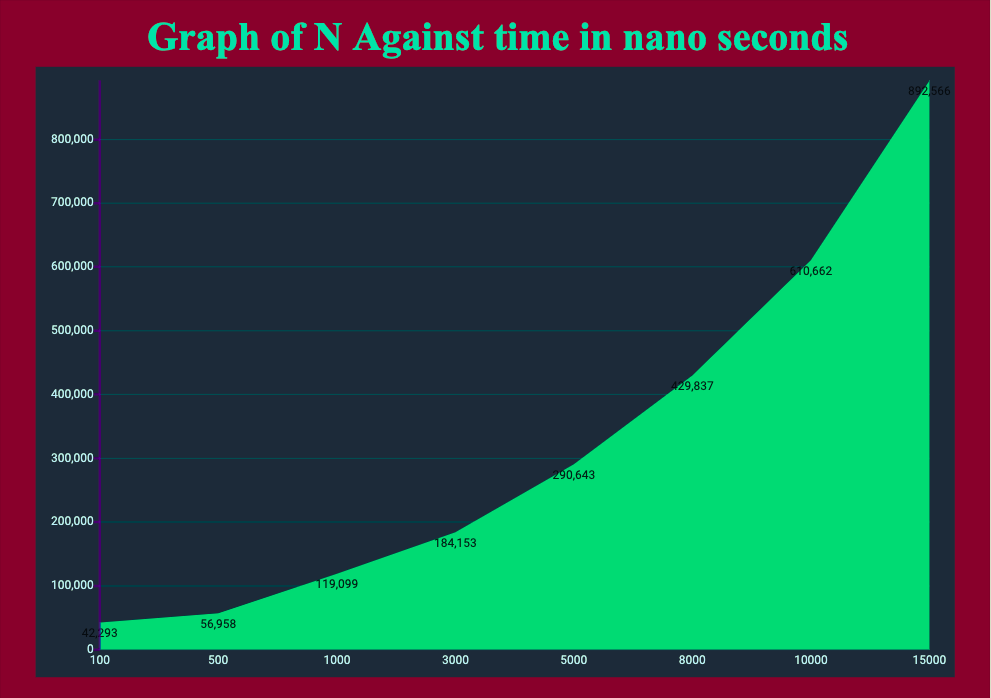
\includegraphics[width=8cm]{images/graphn.png}
\end{figure}

\begin{center}
 \begin{tabular}{||c| c| c||} 
 \hline
 N & M & Time(in nanoseconds) \\ [0.5ex] 
 \hline\hline
 10 & 100 & 31042  \\ 
 \hline
 10 & 500 & 63804  \\ 
 \hline
 10 & 1000 & 71490  \\ 
 \hline
 10 & 3000 & 116213  \\ 
 \hline
  10 & 5000 & 204245  \\ 
 \hline
  10 & 8000 & 368717  \\ 
 \hline
  10 & 10000 & 628989  \\ 
 \hline
  10 & 15000 & 912566  \\  [1ex] 
 \hline
\end{tabular}
\end{center}
\begin{figure}[h]
\caption{Graph of M Against time in nanoseconds\\}
\centering
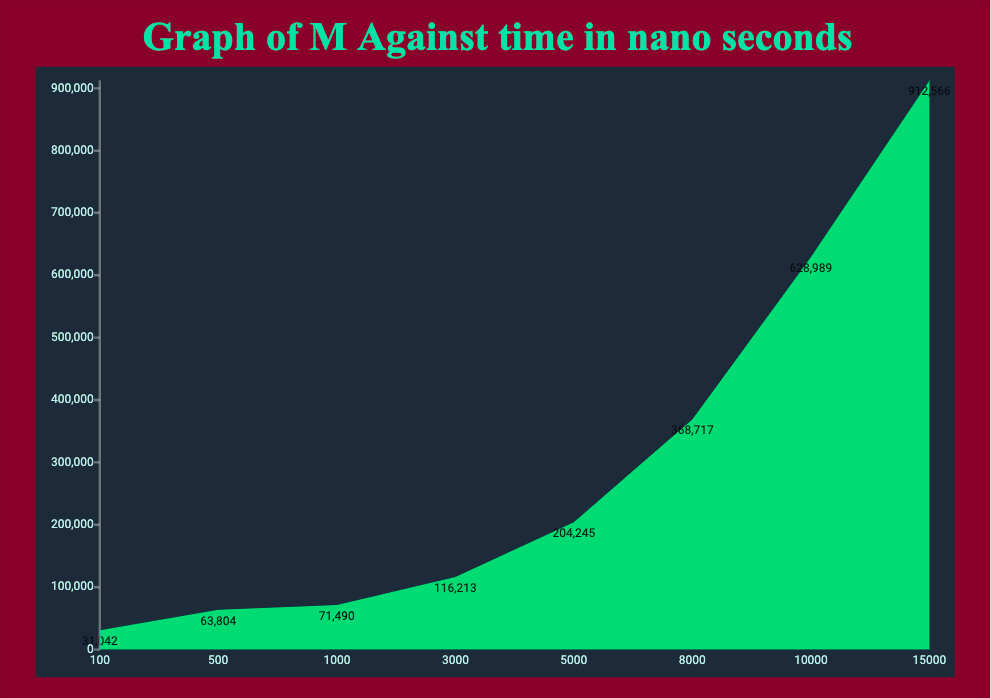
\includegraphics[width=8cm]{images/graphm.png}
\end{figure}

\section{Conclusion}
We can observe that In Dynamic Programming Approach it may consume more space but will have better time-complexity than Brute force approach.

 \section{References}
\color{blue}1.{\url{https://www.geeksforgeeks.org/calculate-xor-1-n/} }\\
2. {\url{https://www.geeksforgeeks.org/dynamic-programming/}}\\
3. Cormen, Leiserson, Rivest, and Stein (2009). Introduction to Algorithms, 3rd edition.

\color{black}
\
\begin{titlepage}
    \begin{center}
        \Huge
        \section*{Appendix}
        \end{center}
         \textbf{Code for implementation of this paper is given below:}
\begin{lstlisting}[language=C++,caption=Code for this paper]
#include<bits/stdc++.h>
using namespace std;
int n,k;
int subsetXOR(int arr[])
{
    int max_ele = arr[0];
    for (int i=1; i<n; i++)
       if (arr[i] > max_ele)
           max_ele = arr[i];
 
    int m = (1 << (int)(log2(max_ele) + 1) ) - 1;
    if( k > m  )
       return 0;
    int dp[n+1][m+1];
    for (int i=0; i<=n; i++)
        for (int j=0; j<=m; j++)
            dp[i][j] = 0;
    dp[0][0] = 1;
 
    // Fill the dp table
    for (int i=1; i<=n; i++)
        {
            for (int j=0; j<=m; j++)
            dp[i][j] = dp[i-1][j] + dp[i-1][j^arr[i-1]];
        }
 
    //  The answer is the number of subset from set
    //  arr[0..n-1] having XOR of elements as k
    return dp[n][k];
}
 
// Driver program to test above function
int main()
{
    cout<<"Enter number of elements"<<endl;
    cin>>n;
    int arr[n];
    cout<<"Enter the elements"<<endl;
    for(int i=0;i<n;i++)
    cin>>arr[i];
    cout<<"Enter value of K"<<endl;
    cin>>k;
    cout << "Count of subsets is " << subsetXOR(arr);
    
}
   
\end{lstlisting}
\end{titlepage}
\end{document}
